\documentclass[11pt,letterpaper]{article}
\usepackage[top=0.85in,left=0.85in,footskip=0.75in]{geometry}
\usepackage{mathpazo}
\usepackage{mdframed}
\usepackage{graphicx}
\usepackage{sectsty}
\allsectionsfont{\normalfont\sffamily\bfseries}
\subsectionfont{\normalfont\sffamily\bfseries}

% cite package, to clean up citations in the main text. Do not remove.
\usepackage{cite}
\usepackage{amsmath}

% To place figures exactly on a page
\usepackage{float}
\usepackage{graphicx}

% Bold the 'Figure #' in the caption and separate it from the title caption with a period
% Captions will be left justified
\usepackage[aboveskip=1pt,font=small,labelfont=bf,labelsep=period,singlelinecheck=off]{caption}

% Strike out
\usepackage[normalem]{ulem}

% Custom BiBTeX style
\bibliographystyle{bibStyle}

% Remove brackets from numbering in List of References
\makeatletter
\renewcommand{\@biblabel}[1]{\quad#1.}
\makeatother

\usepackage{color}
\usepackage[dvipsnames]{xcolor}
\usepackage[colorlinks=true, allcolors=blue]{hyperref}
\usepackage{helvet}

% To define more useful LaTeX commands
\usepackage{xparse}
\usepackage{graphicx}

% Equation referencing
\DeclareDocumentCommand \eref{oooo} {\IfNoValueTF{#2}{Eq. R~(\ref{#1})}{\IfNoValueTF{#3}{Eqs.~(\ref{#1}) and (\ref{#2})}{\IfNoValueTF{#4}{Eqs.~(\ref{#1})-(\ref{#3})}{Eqs.~(\ref{#1})-(\ref{#4})}}}}

% Figure referencing
\DeclareDocumentCommand \fref{ooo} {\IfNoValueTF{#2}{Fig.R~\ref{#1}}{\IfNoValueTF{#3}{Figs.~\ref{#1} and \ref{#2}}{Figs.~\ref{#1}-\ref{#3}}}}
\renewcommand{\thefigure}{R\arabic{figure}} 
\renewcommand{\theequation}{\sffamily R\arabic{equation}} 
\renewcommand{\thetable}{\sffamily R\arabic{table}} 

%% setup the response environment
\mdfdefinestyle{revstyle}{
outerlinewidth=2pt,
bottomline=true,
leftline=true,rightline=true,
topline=true,
font=\small,
skipabove=\baselineskip,
skipbelow=\baselineskip,
roundcorner=10pt,
innertopmargin=0.5em,
innerbottommargin=1em,
splittopskip=1em,
splitbottomskip=1em
}

\mdfdefinestyle{respstyle}{
outerlinewidth=2pt,
bottomline=false,
leftline=false,rightline=false,
topline=false,
font=\small,
backgroundcolor=gray!20,
skipabove=\baselineskip,
skipbelow=\baselineskip,
roundcorner=10pt,
innertopmargin=0.5em,
innerbottommargin=1em,
splittopskip=1em,
splitbottomskip=1em
}

\newmdenv[style=revstyle,frametitle=\sffamily \itshape Reviewer Comment]{review}
\newmdenv[style=respstyle,frametitle=\sffamily \itshape Author Response]{response}
\newmdenv[style=respstyle,frametitle=\sffamily \itshape Author Response: Executive Summary]{responseSummary}

%%%%%%%%%%%%%%%%%%%%%%%%%%%%%%%%%%%%%%%%%%%%%%%%%%%%%%%%
%% END MACROS SECTION%%%%%%%%%%%%%%%%%%%%%%%%%%%%%%%%%%%
%%%%%%%%%%%%%%%%%%%%%%%%%%%%%%%%%%%%%%%%%%%%%%%%%%%%%%%%

\begin{document}
\section*{Response to Reviewer for PONE-D-19-32846 ``Theoretical Investigation of a Genetic Switch for Metabolic Adaptation''}
Kathrin S. Laxhuber\textsuperscript{1},
Muir J. Morrison\textsuperscript{2},
Griffin Chure\textsuperscript{3},
Nathan M. Belliveau\textsuperscript{4},
Charlotte Strandkvist\textsuperscript{5},
Kyle L. Naughton\textsuperscript{6},
Rob Phillips\textsuperscript{2,3$\dagger$}
\vspace{10pt}

\noindent\tiny{
$^1$ Department of Chemistry and Applied Biosciences, ETH Zurich, 8093 Zurich, Switzerland,
$^2$ Department of Physics, California Institute of Technology, Pasadena, CA, USA,
$^3$ Division of Biology and Biological Engineering, California Institute of Technology, Pasadena, CA, USA,
$^4$ Howard Hughes Medical Institute, University of Washington, Seattle, WA, USA,
$^5$ Department of Systems Biology, Harvard Medical School, Boston, MA, USA,
$^6$ Department of Physics and Astronomy, University of Southern California, Los Angeles, CA, USA, $^\dagger$ E-mail: \texttt{phillips@pboc.caltech.edu}}

\begin{responseSummary}
We thank the editor and reviewer for considering our manuscript and
bringing some important points to our attention. The reviewer's comments
significantly improved our work and inspired us to make very interesting
comparisons between the deterministic and stochastic picture of our
system. Furthermore, as rightly suggested by the reviewer, we have now
added experimental data to the manuscript and expanded the author list
to reflect this. Below, we address the reviewer's concerns one-by-one
and indicate where changes were made either to the main text or the
supporting information. Besides these changes, we made a few small
improvements and corrections to the text that had slipped our attention before. We
believe we have resolved the three issues brought up by the reviewer and
hope our manuscript is now ready for publication in PLOS ONE.
\end{responseSummary}

\subsection*{Reviewer \#1}
\begin{review}
In their manuscript "Theoretical investigation of a genetic switch for
metabolic adaptation", Laxhuber and colleagues present a very nice
theoretical analysis of the behavior of the \emph{E. coli} xapABR system, using
both deterministic and stochastic simulations to demonstrate that the
system can show meaningful and important bistability driven by the
activity of the membrane transporter. In general the work is well done,
and it is technically of high quality, but at present I have two
substantial concerns that I think must be addressed in order for the
paper to live up to its potential.
\end{review}

\begin{response}
We thank the reviewer for their careful reading of our work and are
pleased that their impression of the manuscript is favorable overall.
\end{response}

\begin{review}
My first concern is that while the authors present their deterministic
simulations first, and draw many of their conclusions primarily from
those simulations, it seems to me that the use of such simulations is
contra-indicated by the authors' own findings. As both the number of
XapR molecules and mRNA molecules are small integers (likely 10 or
less), treatment of these species as continuous, deterministic
quantities can never be more than a poor approximation. I find this
troublesome for a couple of reasons. First, the authors still treat
their continuous treatment as an apparently 'good' way to model a
genetic switch like that at work at the xapAB promoter; while I find
their analysis insightful, in the end I cannot support such a
recommendation given the stochasticity intrinsic in the low protein and
mRNA copy numbers present here.
\end{review}

\begin{response}
We agree with the concern of the reviewer that in general, deterministic
approximations of systems with such low copy numbers need to be verified. We do not intend to give the general recommendation that a
continuous treatment alone is usually sufficient, and in order to avoid
this, we added some words of warning in the beginning of our
deterministic as well as our stochastic analysis.

Nevertheless, for our system we did successfully test the concordance of the stochastic simulations and the deterministic model. To make this more apparent, we included some additional comparisons of the two
models. We address these in more detail in our responses below,
but to summarize: we added a bifurcation diagram
(Fig~\ref{bifucation}) which illustrates that the stochastic
distributions track the deterministic fixed points very well,
and we compared the stochastic timescales with the solution of the
deterministic model (Fig~\ref{adaptationtime}) and found excellent
agreement there too. 

Even though stochastic fluctuations around the deterministic
trajectories may be large, the stochastic trajectories do still flow to
the fixed points as predicted by the deterministic model.
Hence, the excellent agreement may be surprising or unintuitive at first, but the conclusions we draw from the deterministic phase diagrams turn out to be accurate.

%, except when
%the system is close to either of the bifurcation points in
%Fig~\ref{bifucation}, where it is unsurprising that fluctuations are
%magnified in importance.

Given this concordance, we prefer to start by showing the deterministic case and illustrating our conclusions there before moving on to the stochastic picture. That is because the deterministic phase diagrams have the advantage of providing the reader with a more intuitive understanding of the system than the plots of the results from the stochastic simulation.
\end{response}

\begin{review}
Second, while the authors do technically recapitulate the bistable
behavior of the system in the stochastic version, the bistability seems
based on their description to be quite fragile and not very meaningful,
since it only occurs here for small distances between the lower and
upper fixed points
\end{review}

\begin{response}
We thank the reviewer for bringing this point to our attention, which we
believe to be a misunderstanding that resulted from a poor explanation
in our original text. We believe we have clarified this in the
manuscript, and allow us elaborate here too: Stochastic bimodality occurs
only when two of the three fixed points are close together, or in other
words, when the system is poised ``sufficiently near'' one of the
bifurcation points. This may become clearer when looking at the
bifurcation diagram that we added to our section about hysteresis at the
end of the main text. For convenience, we insert this plot below in
Fig~\ref{bifucation} which addresses what we believe the reviewer is
referring to: only when two of the three fixed points are close do the
stochastic trajectories occupy both fixed points, resulting in
bimodality.

Since this bimodality only occurs for a small region in parameter space,
this actually indicates strong and not fragile bistability. In other
words, the fact that the system does not stochastically ``jump'' to the
other fixed point means that the fixed points are very stable to
stochastic fluctuations. Thus, the switch-like feature is robust:
there are two distinct states that the system can occupy, and only near
the bifurcation points is it likely for stochastic trajectories to
transition between them. Put differently, deterministic bistability does
not need to result in stochastic bimodality, and in fact stochastic
bimodality is contrary to robust bistability.
\end{response}

\begin{figure}[h!]
	\centering
	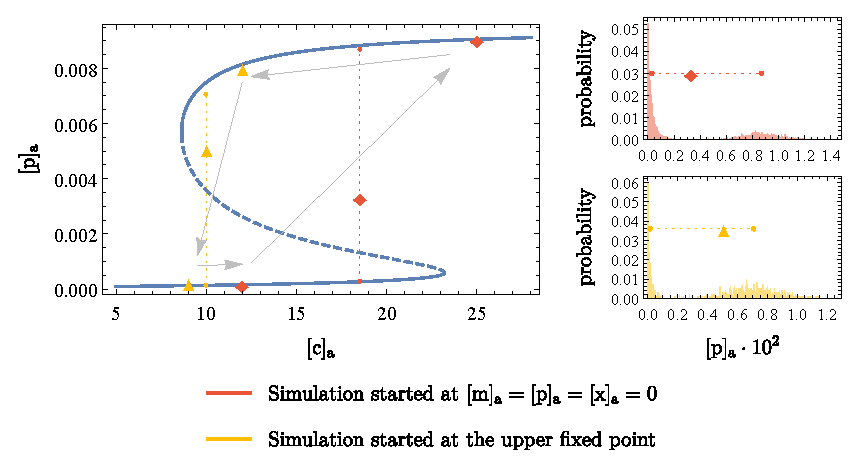
\includegraphics{Fig10_bifurcation.eps}
	\vspace*{0.5em}
	\caption{{\bf Bifurcation diagram showing the hysteresis loop in the stochastic system.}
		The blue line shows the positions of the deterministic fixed points, while the dashed line indicates the instability of the middle one. The orange and yellow points show the mean of the stochastic simulations when started at zero and at the high fixed point, respectively. The positions of the two peaks in the bimodal distributions are indicated by smaller points, connected by dotted lines. To make this clearer, the bimodal distributions themselves are shown on the right. The arrows illustrate the hysteresis loop in the stochastic simulations.}
	\label{bifucation}
\end{figure}

\begin{review}
	(and seems to take an unreasonably long time to switch between states).
\end{review}

\begin{response}
To address the indeed valid point of unreasonable switching times, we
have compared the timescales in our stochastic simulations with those from the
numerical solution of the deterministic model. We find excellent
agreement, as shown in an updated figure in the main text and also below
in Fig~\ref{adaptationtime}. So, again perhaps surprisingly,
stochasticity does not materially alter the mean switching time as
computed from the deterministic picture. Even adding additional
stochasticity through transcriptional bursting (discussed more below)
does not alter the mean switching time, though it does broaden the
distribution of times.
It is possible that this broadening resolves the apparent paradox. Even
if the mean switching time is quite long, a non-negligible fraction of a
population of cells could nevertheless switch on a shorter time-scale,
especially with inclusion of extra stochasticity beyond what we have
explicitly considered.
\end{response}

	\begin{figure}[h!]
		\centering
		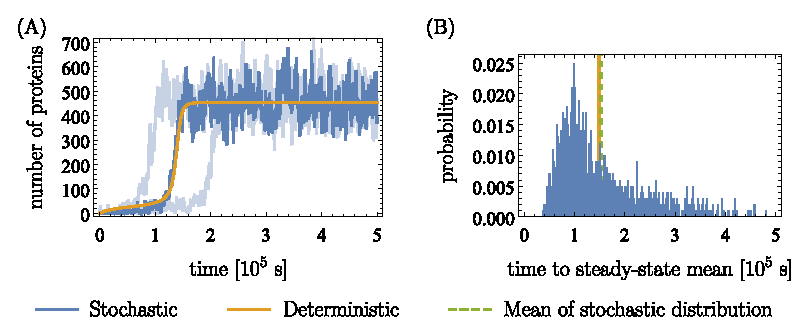
\includegraphics{Fig9_evolution.eps}
		\vspace*{0.5em}
		\caption{{\bf Stochastic and deterministic time evolution of protein (XapA/XapB) and adaptation time.}
			(A) Blue shows the results from one typical run of the stochastic simulation, light blue shows two more extreme runs, and orange shows the trajectory obtained from solving the deterministic ODE's. The simulation was started
			at an mRNA, protein and intracellular xanthosine count of 0. The
			extracellular xanthosine concentration was chosen to be
			$\mathrm{[c]_a} = 25$. (B) Blue shows the time until 90\% of the protein concentration at the upper fixed point was reached in 1000 runs of the simulation (same conditions as (A)). The orange line shows the corresponding deterministic time. The green dashed line right next to it indicated the mean of the blue distribution.}
		\label{adaptationtime}
	\end{figure}

\begin{review}
I think the authors are likely correct in their assertion that they
underestimate the amount of noise in the system due to not including
transcriptional and translational bursting, and that the transition
rates would likely be faster, but this gives no idea of how *much*
faster, and thus it seems premature to simply declare victory and move
on.
\end{review}

\begin{response}
This is a very reasonable concern which we have investigated more
thoroughly now. We added rather strong transcriptional bursting to our
simulation and do not find qualitative changes in the results. In
particular, fluctuations around the mean become larger and, accordingly,
distributions broader. Furthermore, bimodality begins to appear for
lower values of the extracellular xanthosine concentration. Very
interestingly, the change in the \emph{mean} transition time between the
stable fixed points is negligible. However, the \emph{variance} in this
time across many runs of the simulation becomes larger and the
\emph{peak} of the distribution shifts to shorter times. We have
included two new figures in the SI discussing these results (Figs. 6 and
7), along with discussion there and in the main text.
%	Below, we also show the two new figures from S1 Text that illustrate the similarities and differences between the simulation with and without transcriptional bursting.
\end{response}

%\begin{figure}
%	\centering
%	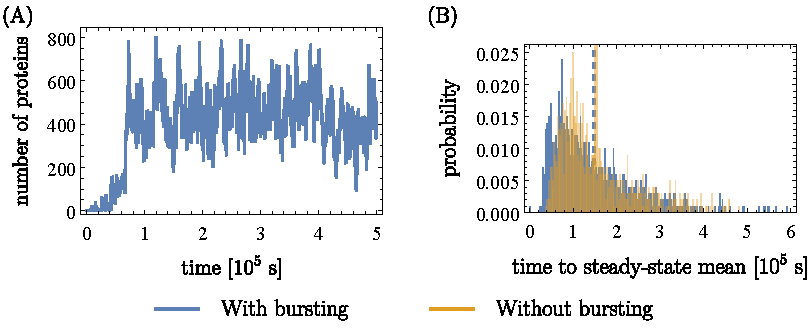
\includegraphics[width=1\textwidth]{FigSI6_7.pdf}
%	\caption{{\bf Time evolution and adaptation times from the stochastic simulation when transcriptional bursting is included.}
%		(A) shows the time evolution from one run of the simulation. The simulation was started
%		at an mRNA, protein and intracellular xanthosine count of 0. The
%		extracellular xanthosine concentration was chosen to be
%		$\n{[c]_a} = 25$. (B) Blue shows the time until 90\% of the protein concentration at the upper fixed point was reached in 1000 runs of the simulation (same conditions as (A)). The distribution from the main text (without bursting) is shown in orange for comparison.}
%	\label{evolbursts}
%\end{figure}
%
%\begin{figure}
%	\centering
%	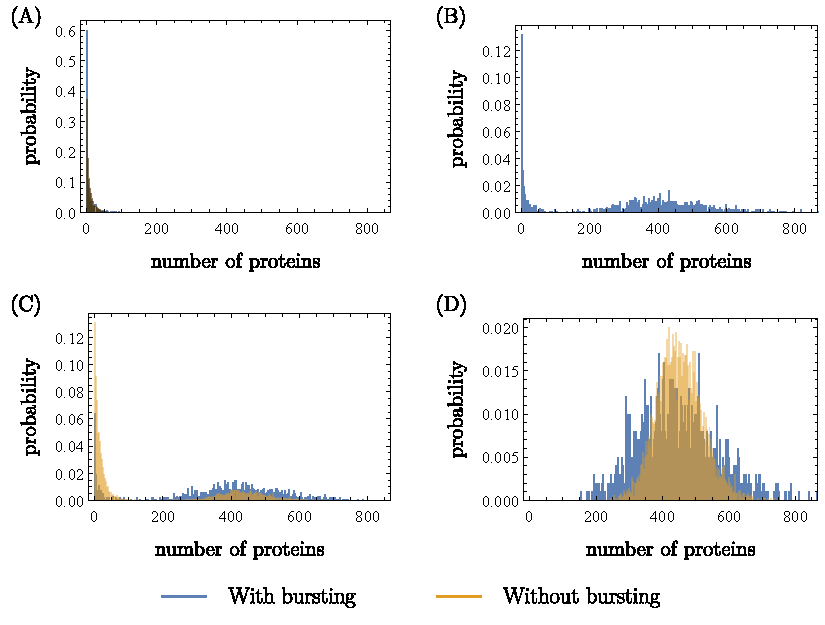
\includegraphics[width=1\textwidth]{FigSI6_7_2.pdf}
%	\caption{{\bf Distributions from the stochastic simulation when transcriptional bursting is included.}
%		Blue shows the distributions from the simulation with bursts, orange shows those without bursts from the main text for comparison. The following values of $\mathrm{[c]_a}$ were used: (A) $\n{[c]_a}=12$, (B) $\n{[c]_a}=17.5$ (not shown in main text), (C) $\mathrm{[c]_a}=18.5$, and (D) $\mathrm{[c]_a}=25$ (recall $\n{[c]_{a}} \defeq \frac{c}{K_{\n{a}}}$,
%		$K_{\n{a}} = 5 \cdot 10^{-5} \unit{M}$). All other parameters are as in the table in the main text, and the simulation
%		was run 1000 times for $10^6 \unit{s}$ each (simulated time) and
%		started at a mRNA, protein and intracellular xanthosine count of 0.}
%	\label{distbursts}
%\end{figure} 

\begin{review}
My recommendation would be that the authors put in some more cautionary words about the applicability of the continuous model, and ideally spend a little more time characterizing the discrete model. in terms of switching times, parameters that give rise to bimodal behavior, effects of incorporating reasonable amounts of transcriptional bursting, etc. Some more direct comparisons of the behavior of the two models in similar ranges of parameters space would also likely be enlightening.
\end{review}

\begin{response}
We hope that we have addressed all these points in our responses above
and shortly summarize here: We put in some cautionary words about the
general usage of continuous models (beginning of sections on deterministic as well as stochastic results) and demonstrated that for our system
and the conclusions we draw, the continuous model is surprisingly appropriate (bifurcation diagram and time evolution, end of results section).
Furthermore, we extended our characterization of the stochastic model as
suggested by investigating the distribution of adaptation/switching
times (end of results section) as well as by incorporating transcriptional bursting in our
simulation (end of section C in S1 Text). The deterministic and stochastic model are now directly
compared (for the same set of parameters) in the bifurcation diagram as
well as in terms of their adaptation/switching times.
\end{response}

\begin{review}
My other major difficulty here is that essentially all of the work is
premised on reference 22, which is 'unpublished data.' This is the only
experimental evidence given for the bistability of xapAB expression,
justification of many of the model parameters, experimentally expected
switching timescales, etc. It is impossible to properly interpret the
present work, either for the purposes of review or from the viewpoint of
an interested reader, without availability of those data, which either
ought to be their own independent publication or ought to be included
with this one.
\end{review}

\begin{response}
With further consideration, we agree with the reviewer that we relied
rather heavily on this unpublished data and that it is therefore
essential to make the experimental data available.
We have opted to include the data with this publication rather than
separately. For this reason, we have added Griffin Chure, Nathan Belliveau, Charlotte Strandkvist, and Kyle Naughton to the author list, who collected or were involved in collecting the data. We have added a new section, ``experimental motivation,'' in
the beginning of the main text which discusses the main features of the
data that are relevant for our model. Furthermore, we added a section on
the materials and experimental methods at the end of S1 Text (section
E).
The raw data is
publicly available at DOI: 10.5281/zenodo.3695049.
\end{response}

%\begin{figure}[h]
%    \centering{
    %\includegraphics{figure_path}
%     \caption{\textbf{Figure caption.}}
%    \label{fig:figlabel}}
% \end{figure}


\bibliography{library}

\end{document}
